\chapter{The Vault: Assembling Related Source Code Artifacts}%
\label{chp:vault}

In the previous chapters, we have outlined the different challenges in making
Software Heritage a universal software mining platform. By studying the needs
of researchers in the fields of empirical software engineering who perform
studies on software repositories, it is possible to get a good sense of the
best ways the archive could become useful as a research platform.

However, building the universal platform constitutes a huge endeavor that has
to be done incrementally. As we cannot aim to cover most use cases overnight,
we should instead prioritize features that are immediately useful to
researchers so that they can start using the building blocks we provide in
their work. Aside from driving up engagement with the research community, this
also helps identify the main pain points they encounter, which in turn can
plot the roadmap in the steps we take to alleviate them.

The very first step that has to be taken to make the archive usable as a
bare-bones platform is to provide a simple way to retrieve single artifacts or
logical groups of artifacts from our own storage. While this cannot necessarily
make large-scale analysis possible, this could at least be used for some
smaller-scale experiments and prototypes.

For single artifacts, the Software Heritage
API\footnote{\url{https://archive.softwareheritage.org/api/}} already somewhat
covers this use case: using the \gls{SWHID} of an object, it is possible to
retrieve its associated data as stored in the archive. This use case is
relevant for researchers because it provides a first form of availability: many
studies can be conducted using only \gls{VCS} object identifiers; the archive
is able to complement these studies by allowing readers to retrieve the actual
objects behind these identifiers instead of putting on researchers the burden
to provide the full artifacts themselves.
As an example, the following HTTP GET request can be used to get the revision
\texttt{swh:1:rev:aafb16d69fd30ff58afdd69036a26047f3aebdc6}:

\vspace{1em}

\begin{minipage}{0.96\textwidth}
\begin{minted}[fontsize=\footnotesize]{bash}
% curl 'https://archive.softwareheritage.org/api/1/revision/
        aafb16d69fd30ff58afdd69036a26047f3aebdc6/'
\end{minted}
\begin{minted}[fontsize=\footnotesize]{python}
{
    "id": "aafb16d69fd30ff58afdd69036a26047f3aebdc6",
    "message": "Merge branch 'master' into pr/584\n",
    "author": {
        "email": "nicolas.dandrimont@crans.org",
        "fullname": "Nicolas Dandrimont <nicolas.dandrimont@crans.org>",
        "name": "Nicolas Dandrimont"
    },
    "date": "2014-08-18T18:18:25+02:00",
    "directory": "9f2e5898e00a66e6ac11033959d7e05b1593353b",
    "metadata": {},
    "parents": [ ... ]
    [ ... ]
}
\end{minted}
\end{minipage}

\vspace{1em}

While this works well to check the status of a single artifact, it is tedious
to use for more complex use cases. Even for relatively small-scale experiments
on a single repository, researchers will generally want to fetch at least an
entire source code tree.  In this chapter, we introduce a new component in the
Software Heritage infrastructure to fetch entire groups of software artifacts
at once: the Vault.

\section{Design}

A core design choice in the \SWH{} archive is to deduplicate every single
software artifact and consolidate them in a shared storage. While this has a
lot of interesting properties for archival (outlined in
\cref{sec:consolidation}), like traceability and reduced storage space, it
comes with an important trade-off: artifacts contained in a single repository
are spread out all over the archive during the ingestion process, and the
retrieved \gls{VCS} bundles and packages are then thrown away. This means that
retrieving a repository from the archive requires reassembling all its
components and putting them back in a compact, downloadable format.

The general goal of the Vault is to provide a way to assemble logical groups of
related software artifacts into a single \emph{bundle}. This assembling process
is called ``cooking''. It takes a single \gls{SWHID} as an input and traverses
the Merkle DAG to assemble all the artifacts that are \emph{reachable} in the
subgraph rooted at that artifact.

Concretely, this means that cooking a directory will assemble all its
subdirectories and blobs, whereas for a revision it will walk down the
entire chain of parent revisions and assemble all their associated root
directories (and, recursively, their own subdirectories and blobs).
Once the objects are cooked, they are assembled in a suitable format that is
specific to the type of object that was cooked, respectively:

\begin{itemize}
    \item for \textbf{directories}, the entire file hierarchy contained in the
        directory is cooked as a \emph{tarball}, a file format which combines
        and compresses multiple files and directories.
    \item for \textbf{revisions}, the entire commit chain of the revision's
        ancestors is put in an empty \emph{git repository}, along with all the
        files and directories they contain.
    \item for \textbf{snapshots}, each branch and tag in the snapshot is
        followed to get the entire commit graph of the snapshotted repository,
        and all objects are similarly written to an empty git repository.
\end{itemize}

In essence, cooking a snapshot allows one to ``clone'' an entire repository
stored in the archive as a git repository. Because this cooking process can
take some time, the Vault is designed as a two-step cache. First, the cooking
step asynchronously prepares the bundle of artifacts and writes it as a single
file in its internal storage, then notifies the requester that the object is
ready for retrieval. After doing so, the Vault can efficiently serve the
artifact from its internal storage as a static file via HTTP, in effect acting
as a cache for the bundle cooking process.

The cooking process is deterministic: its input is a \gls{SWHID}, which,
because of the properties of the Merkle DAG, always refers to the same sub-DAG
of software artifacts\footnote{In theory this is not always true because the
data model can contain holes of artifacts that were not retrieved at first,
but then found in a later crawl. This edge case is largely ignored for now in
the archive because of the added complexity handling it would incur.}. This
means that the cooking process can be deduplicated: if some artifact
experiences a sudden surge in popularity (because it disappeared from its
hosting place or was publicized through other means), many users will try
to request it at once. There is no need to restart the cooking process for
each user; instead, by keying each bundle with the \gls{SWHID} it
assembles, the process can be shared so that the cooking of each bundle
happens only once.

% \begin{figure}[b]
%     \centering
%     \begin{tikzpicture}[scale=1.4]
	\begin{pgfonlayer}{nodelayer}
		\node [style=server, fill={blue!20!white}] (0) at (0, 0) {Backend};
		\node [style=server, fill={green!30!white}] (1) at (4, 0) {Cooker};
		\node [style=server, fill={green!30!white}] (2) at (4, 1.5) {Cooker};
		\node [style=server, fill={green!30!white}] (3) at (4, -1.5) {Cooker};
		\node [style=server, fill={gray!30!white}] (4) at (0, 2) {Database};
		\node [style=server, fill={rgb,255: red,198; green,192; blue,193}] (5) at (0, -2) {Storage};
		\node [style=server] (6) at (-2, 0) {Web \\ Server};
		\node [style=server] (7) at (-4, 0) {User};
		\node [style=server] (8) at (2, 0) {Task \\ Queue};
	\end{pgfonlayer}
	\begin{pgfonlayer}{edgelayer}
		\draw (0) to (4);
		\draw (0) to (5);
		\draw (6) to (0);
		\draw (7) to (6);
		\draw (2) to (8);
		\draw (8) to (1);
		\draw (8) to (3);
		\draw (0) to (8);
	\end{pgfonlayer}
\end{tikzpicture}

%     \caption{Architecture of the Vault Service}%
%     \label{fig:vault-design}
% \end{figure}

\begin{figure}
  \centering
  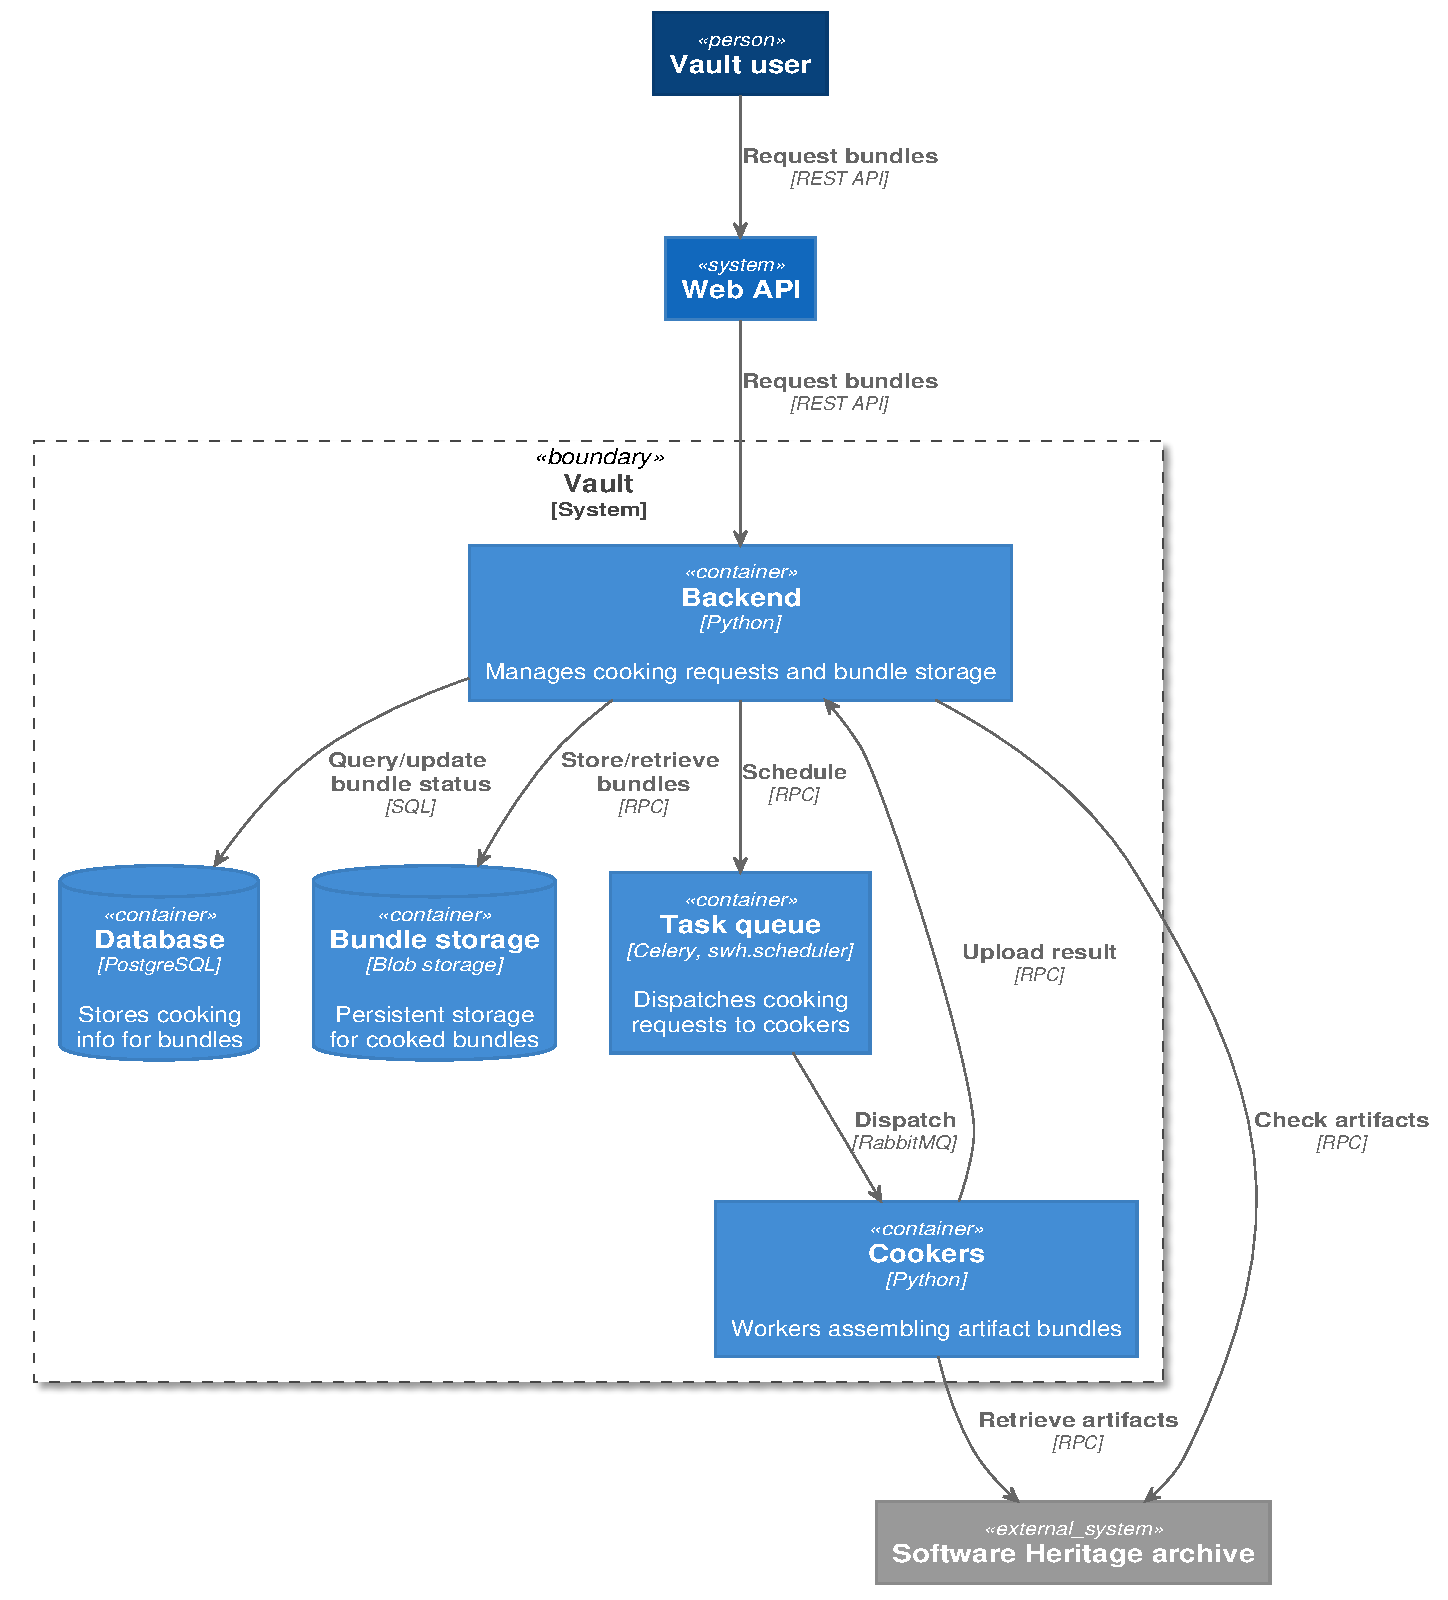
\includegraphics[width=\linewidth]{img/vault/arch-container}
  \caption{C4 architecture diagram of the Software Heritage Vault.}%
  \label{fig:vault-arch}
\end{figure}

\Cref{fig:vault-arch} shows the architecture of the service as a C4
diagram~\cite{brown2018c4}. It is centered
around the Vault backend, which directly communicates with a database where the
status of the bundles is kept up-to-date, as well as an internal storage where
the bundles can be written and from which they can be later efficiently
retrieved. It can also distribute tasks to a worker pool of ``cookers'' which
retrieve and assemble artifacts from the main Software Heritage database.  This
design ensures a low coupling between the backend and the cookers, which allows
the cooking capacity to be horizontally scaled in a straightforward manner by
having new resources simply register themselves in the task queue.

In a typical workflow, a user requests the cooking of a bundle from the web
API,\footnote{\url{https://docs.softwareheritage.org/devel/swh-vault/api.html}}
which forwards the cooking request to the Vault backend. The backend then tries
to add this cooking request to the database; if no cooking request for this
artifact is already present as pending or completed, it asynchronously
dispatches the task to one of the ``cooker'' servers through a task queue. It
then immediately returns a task identifier to the user. While the cooking
process is pending, the cookers periodically send requests to the backend with
the current progress of the cooking; this progress is written to the database
and can be requested at any time by the user. Once the cooking process is
complete, the cookers stream the resulting bundle to the backend which writes
it in its storage. The backend then updates the database to mark the bundle as
ready for retrieval, notifying the users who can then send a download request
to efficiently retrieve it.

\section{Cooking process and bundle formats}

The cooking process itself has many design considerations that impact ease of
retrieval and ease of use. Being able to cook bundles efficiently is key for
this process to be practical for large scale analysis, as researchers can
sometimes request thousands of repositories to use for a single study. In this
section we look at the ways to efficiently assemble the two main kinds of
bundles: directories and commit graphs (for revisions and snapshots).

\subsection{Cooking directories}

Cooking directories from the main archive storage is a relatively simple
endeavor: the children of each directory can be recursively retrieved by
making several directory listing queries to the storage. As the directory
traversal happens in a depth-first fashion, the directory names are pushed onto
a stack; during the traversal, the full path of the current object is obtained
by reading the contents of the stack.

As fetching blobs individually is generally expensive, the blob retrieval
requests to the storage are \emph{batched}: instead of fetching the blobs
during the recursive directory traversal, they are added to an asynchronous
fetching queue, which retrieves the files by batches of a thousand items. These
files are then written to the tarball output, as archives in the tar format can
be built incrementally.

\begin{algorithm}[t]
    \begin{algorithmic}
        \Function{FetchDirRec}{$Q,~\mathit{swhid},~\mathit{path}$}
        \ForAll{$c \in \Call{Storage.GetChildren}{\mathit{swhid}}$}
            \State $n \gets \Call{name}{c}$
            \State $p \gets \mathit{path} + "/" + n$
            \If {\Call{type}{c} $=$ \texttt{DIRECTORY}}
                \State $\Call{FetchDirRec}{Q,~c,~p}$
            \Else
                \State add $(c, p)$ to $Q$
            \EndIf
        \EndFor
        \EndFunction

        \Function{CookDir}{$\mathit{swhid}$}
        \State $Q \gets$ empty queue  \Comment{Queue of blobs to fetch}
        \State $T \gets$ empty tarball  \Comment{Output tarball}
        \State $\Call{FetchDirRec}{Q,~\mathit{swhid}, ""}$
        \State $C \gets \Call{FetchContentsBatched}{Q, 1000}$
        \ForAll{$(c, p) \in C$}
            \State write $c$ in $T$ at path $p$
        \EndFor
        \State \Return $T$
        \EndFunction
    \end{algorithmic}

    \caption{Recursively ``cook'' a directory in a tarball.}%
    \label{algo:cooking-directory}
\end{algorithm}


\Cref{algo:cooking-directory} shows the recursive directory cooking
algorithm.
In this algorithm, fetching blobs is \emph{embarrassingly
parallel} and can be scaled up at will. However, building the queue of blobs
to fetch is done in a sequential fashion with several directory listing
requests sent to the archive storage, each request being directly dependent on
the SWHID retrieved by the previous requests.

This bottleneck massively increases the number of round-trips between the cooker
and the storage. This behavior could be improved in two ways. The first
would be to replace the depth-first traversal by a parallel breadth-first
search, reducing the number of sequential round-trips from $O(n)$ to $O(h)$
(the height of the directory tree). While this improves throughput by reducing
total latency, it still requires a large number of round-trips.
Another option would be to compute the entire subtree of the directory
recursively directly in the storage side, then return the file hierarchy in a
single response. However, our current storage system backed by PostgreSQL
cannot efficiently compute these requests and still has to do round-trips with
the database itself. Later in the thesis (\cref{chp:graph-compression}), we
will explore ways based on graph compression to efficiently reply to those
recursive ``vault queries'', i.e., being able to quickly compute the entire
subgraph reachable from a node.

\subsection{Cooking revisions and snapshots}

The standard format used to cook directories is relatively straightforward: a
source code tree can easily be exploited for software mining when distributed
as a compressed tarball. When the subgraph reachable from an artifact includes
revision chains however, as is the case when cooking revisions and snapshots,
there is no natural format in which the commit graph can be distributed; the
best format to use requires further evaluation.

One simple format would be to ``flatten'' the entire chain: a directory at the
root would contain one subdirectory per revision, then each of these would
contain the state of the source tree for the given revision. While cooking
bundles in this format is easy to implement using the algorithm described in
the previous section, the output bundle will be of considerable size:
flattening the revisions removes all the Merkle DAG deduplication, as each new
commit copies the entire source tree. While hard links and symbolic
links could be valid ways to implement deduplication for these objects, the
former are not portable, and the latter get in the way of studies which rely on
trustworthy file modes and types.

A preferable option is to export these bundles directly as Git repositories.
Software mining researchers are already accustomed to working with these
repository formats and thus generally have tools already available to extract
relevant data from them. Because Git is the most popular \gls{VCS}, it makes
sense to provide a way to export revisions and snapshot bundles as Git bundles.

To export archived artifacts as a Git repository, we first investigated the
format used by \texttt{git
fast-import},\footnote{\url{https://git-scm.com/docs/git-fast-import}} designed
to be an interchange format between \glspl{VCS} and which can efficiently
import data into a git repository.
This format contains a stream of ``commands'' which describe all the Git
objects to import (tags, commits, trees and blobs), and is used by many
\gls{VCS} converters. Implementing this cooker exposed a few limitations of the
format itself: poor documentation, unfriendly interface due to its relatively
uncommon usage, lossiness (no tagged trees and incomplete handling of signed
tags) and large output (the format was not meant for long term storage and has
no built in delta-compression of blobs).
Most importantly, it is very expensive to export from the archive, because the
commits are represented as a list of changes between one state to the other.
Generating revisions under this format requires computing diffs between
consecutive commits, which is expensive and hard to parallelize.

Yet a better approach is to create a cooker for Git \emph{bare}
repositories\footnote{\url{https://git-scm.com/book/en/v2/Git-on-the-Server-Getting-Git-on-a-Server}},
i.e., a tarball of the internal data store of a Git repository which can be
easily cloned with the Git command line. Implementing this cooker is relatively
straightforward: it involves listing all the objects reachable from the
revision or snapshot artifact, then directly writing each object in the Git
object storage. These objects can then be delta-compressed together using
\texttt{git repack}.

\section{Discussion}

The Vault is generally an efficient way to retrieve substantial lists of
repositories or source code trees from the archive. A moderately sized
repository with around $\approx 390$ commits takes around 7 minutes, while its
source code tree of $\approx 60$ files takes 19 seconds. By extrapolating these
benchmarks and from our own experiments, the Vault is suitable to retrieve up
to tens of thousands of directories and thousands of repositories from the
archive in a reasonable time (between a few hours and a few days). This service
offers a first rudimentary way of performing software mining studies on data
extracted from the archive.

One possible future direction for this work would be to ``pre-cook'' a large
number of objects according to certain heuristics, as a way to decrease cooking
latency. While we cannot anticipate which objects would be the most relevant to
study for researchers, it is likely that some particular objects such as
revisions pointed by releases or the latest available source tree of each
repository would be of particular interest to them, and thus a reasonable
heuristic for pre-cooking.

The main advantage of retrieving repositories using the Vault is that their
format is common (simple directories and Git repositories), allowing
researchers to use their own day-to-day tools for analysis, without having to
write custom programs specifically for running experiments on the archive. This
advantage comes at the loss of the deduplication that was present in the
original data model: while the Vault can be used to analyze repositories one by
one, all the data sharing links between the repositories is lost. Aside from
having implications on space usage, it also makes it challenging for
researchers to study the duplication relationships between the different
artifacts. More generally, this approach is not suitable for exhaustive or
macro studies on the entire software commons.

A final caveat is that using the Vault to retrieve repositories is frictional
and requires some upfront work to retrieve repositories that can be harder than
to simply clone the original repositories themselves. The Vault is still
valuable for these use cases, as the original repositories are not guaranteed to
still be available or even stable over time due to history rewrites, however it
leaves significant room for improvement.  The next chapter tries to bridge the
gap between simplicity and low friction for small-scale mining studies by
exploring another way of making repositories available for use with day-to-day
CLI utilities while requiring less setup.

% \TODO{more numbers. what storage impact? how long would it take to fetch
% everything?}
% "I think that if you turn the few examples mentioned above in TODO about
% cooking time (and maybe add some more, in order to have ~5 repo sizes
% described) it would be good enough in terms of numbers"
